The goal of this chapter is to give a description of the \textit{Bacco} protocol and to discuss the
implementation choices that were made in order to deploy it. This is achieved using a top-down ordering for the level
of detail, meaning that the overview of the network is presented before its specifics.

\section{Overview}
The network is built upon 3 fundamental categories of devices:

\begin{description}[font=$\bullet$~\normalfont\scshape\color{blue!50!black}]
    \item [Sender node] - collects data and sends it to the gateway using LoRa
    \item [Repeater node] - listens to the incoming LoRa messages form Senders and sends them to a Gateway \footnote{The use of Repeaters where
physical obstacles compromise the integrity of the signals is of very high
relevance in agricultural contexts, since natural barriers such as hills can easily block \gls{VHF} radio signals.}
    \item [Gateway node] - collects data coming from the sender nodes and sends it to the web server using the FTP
        protocol over a mobile network such as \gls{GSM} or \gls{LTE}.. This node has
        also the role of coorinating and syncronizing Sender nodes. It can be optionally configured to perform pre-processing operations (e.g.\ filtering, smoothing, interpolation ...) on the incoming data
    \item [Web server] - receives data coming from the gateways through FTP, elaborates it and makes it available
        through a self-hosted web application
\end{description}

\begin{figure}[ht]
    \centering
    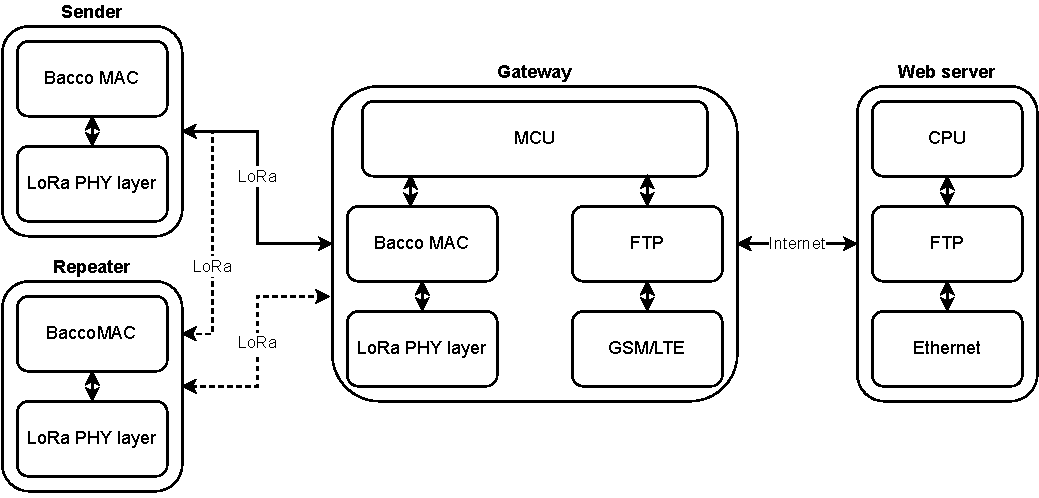
\includegraphics[width=1.0\textwidth]{uml/network_stack.pdf}
    \caption{Schematic representation of the protocols involved}
    \label{network stack img}
\end{figure}

\section{Topology}
The network has a star-of-stars topology, in which the zeroth level is occupied by the Web server, the first level by the
Gateways and Repeaters, and the second level contains the Senders.
Figure \ref{network topology img} shows the type of devices that are involved and their communication schema. \\
The structure is equivalent to a tree, hence we can define a hierarchy of nodes. The root node is the central web server
and its children nodes are the Gateways. All sender nodes are children of either a Gateway or a Repeater and have to
chlidren, so they correspond to the leaves of the tree.

\begin{figure}[ht]
    \centering
    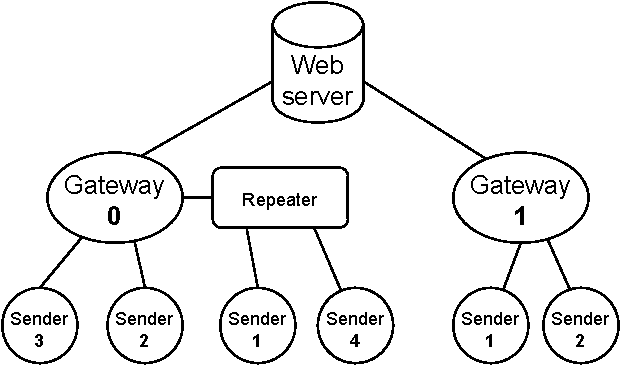
\includegraphics[width=350pt]{uml/network_topology.pdf}
    \caption{Network topology}
    \label{network topology img}
\end{figure}

\section{Addressing}
The addressing scheme follows from the hierarchical structure of the network.\\
A first description of the addressing algorithm is given in the case where there's a fixed number of nodes connected to the
network. Later the procedure will be extended in order to achieve the addition or removal of nodes from the network.
Note that since repeaters do not modify the repeated message (see \cite{DESCRIZIONE DEI RIPETITORI} for a detailed
desription), they are transparent to the other nodes ad thus they will be treated as straight edges by the addressing
algoritm. Note also that since there is only one central Web Server, it is redundant to assign it an identifier.

\subsection{Static addressing}
In order to uniquely identify each node in a static network represented as a tree, we can apply the following procedure:
\begin{itemize}
    \item{May $T$ be a tree and may $r$ be its root node}
    \item{May $\{T_{i}\}$ be a forest of substrees with cardinality of $I$, where $T_{i}$ is a subtree rooted in the child node
        $i$ of $r$, and $I$ is equal to the degree of $r$ }
    \item{For each root node $i$, assing it an identifier that is unique among the other $i$s. In particular the integers
        contained in the interval $\[1,I\]$ will be used to represent each node}
    \item{For each $T_{i}$ apply the same procedure from the first step in a recursive way}
    \item{After applying this algorithm to every possible subtree down to the leaves, each node will have a unique
        identifier among its sibiling nodes}
    \item{Now, to get a unique identifier among all the network for every node, we can concatenate the identifiers
        generated by the algorithm for each ancestors of the node, starting from the root and traversing the tree form parent to child}
\end{itemize}

Each Gateway is manually given a static and unique identifier based on its physical location in the range $\[0,65535\]$.
The maximun number of Sender nodes connected to a single Gateway is limited to 256 \footnote{This choice is influenced
by the current Italian regulations\cite{CITAZIONE PARAGRAFO REGOLAMENTAZIONE CHE
DEVO ANCORA SCRIVERE} \cite{gazzetta_potenza_868} on duty cycle for the 868MHz band and the fact that most agricultural contexts do not require a huge amount of sensors}.

\section{Distribution of transmission activity}
The LoRa PHY protocol does not cover the matter of sharing the communication link between multiple
connected deivices, thus it is necessary to define a method for doing so, in order to minimize interference and achieve
a realiable exchange of information. Many techniques can be applied in the domain of both time and frequency. \\
The Bacco protocol distributes the activity on the channel over time using slots reserved for each Sender, using a
concept that was first introduced by the AlohaNet\cite{alohanet} protocol. The slots are equally distributed between
the Senders, and the start of the frame is function of the identifier. The time delay between transmissions of each Sender is
a constant value and it is called a cycle. At the end of each cycle, a slot is reserved for the Gateway to upload the
data received from the Sender nodes to the Web Server.\\
To make this possible, a 

\subsection{Dynamic addressing}
Dynamic addressing is achieved through the 

Addressing of Sender nodes can be managed dynamically by the corresponding Gateway in order to seamlessly integrate new sensors into the network.

\section{Interference mitigation techniques}
- CAD
- IQ inversion


\begin{figure}[ht]
    \centering
    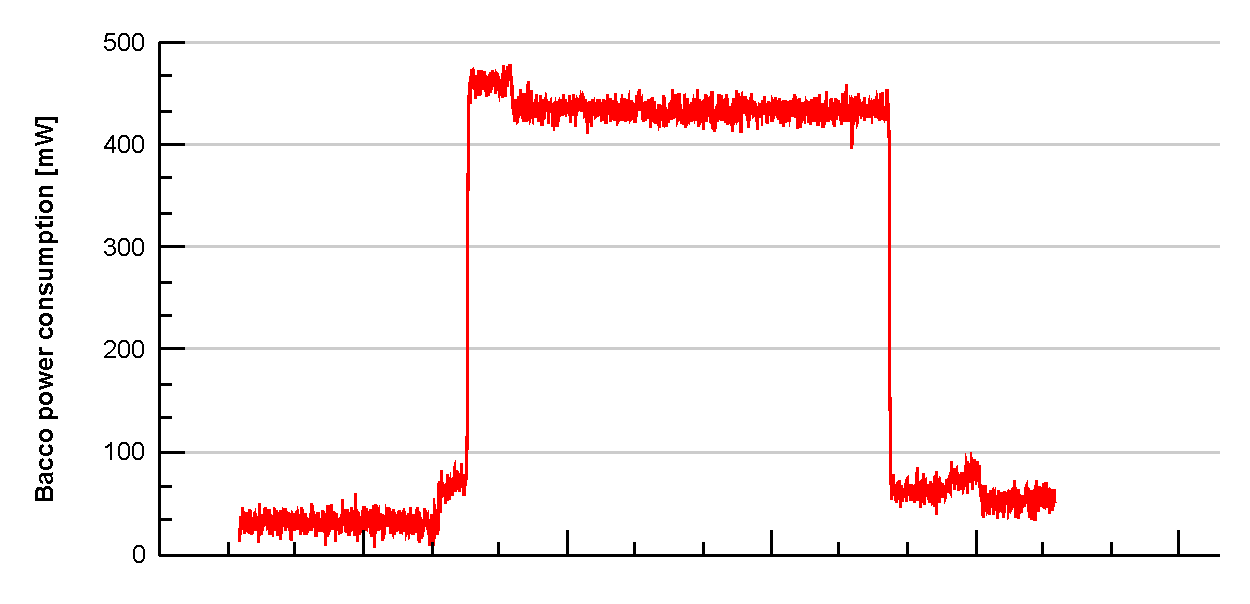
\includegraphics[width=1.0\textwidth]{images/bacco_SF7_14dbm_125khz_power.pdf}
    \caption{Power draw during transmission of a Bacco packet with payload size of 15 bytes, using SF7, 14dBm, 125kHz bandwidth}
    \label{bacco SF7}
\end{figure}
delta time is 51.6ms and total energy is 21.3mJ

\begin{figure}[ht]
    \centering
    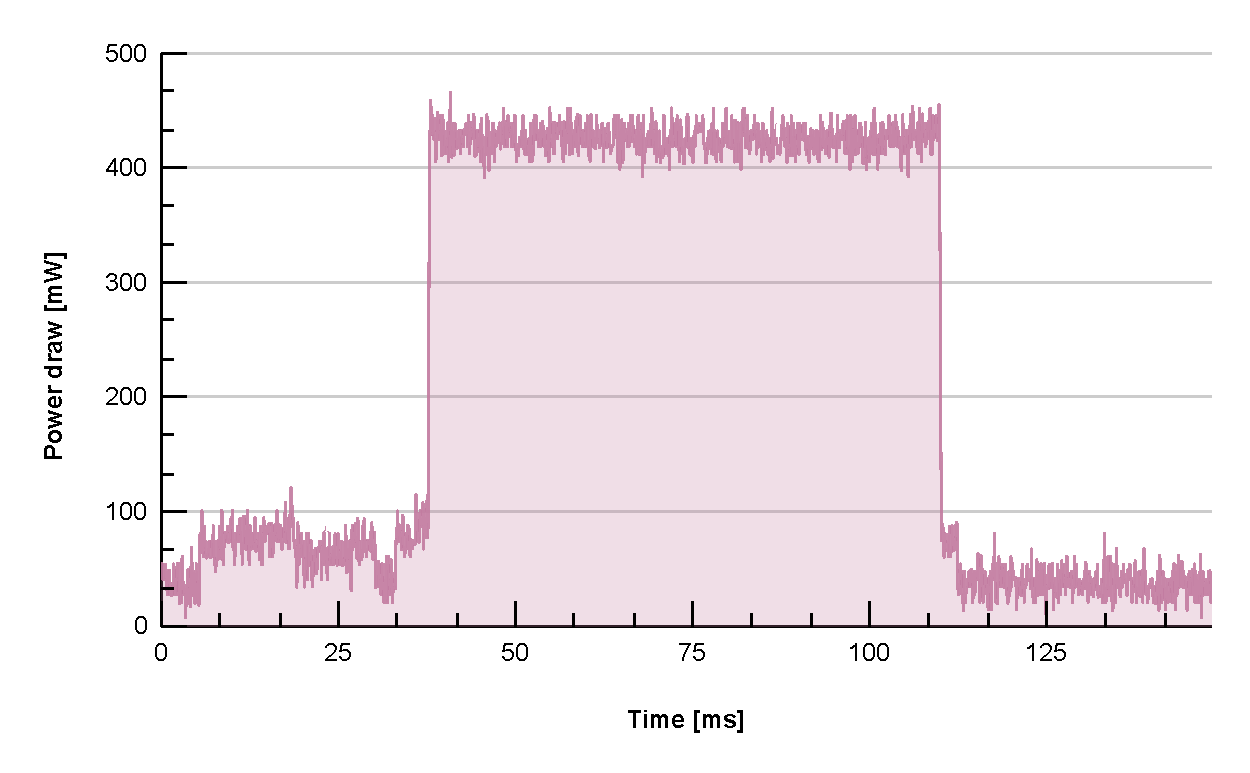
\includegraphics[width=1.0\textwidth]{images/lorawan_SF7_14dbm_125khz_power.pdf}
    \caption{Power draw during transmission of a LoRaWAN packet with payload size of 15 bytes, using SF7, 14dBm, 125kHz bandwidth}
    \label{LoRaWAN SF7}
\end{figure}
delta time is 71.8ms and total energy is 30.8mJ
